\section{Hosting}

Both the backend and frontend were hosted on Render \cite{render}. I chose
Render as a good low cost option for hosting the web service as it offers a free
trial period, constant uptime and backups. A feature I particularly liked was
the ability for the server to instantly deploy whenever I pushed a commit
through to github, if the deployment on render failed then it would revert back
to the previous instance meaning the website was never down. 

I have two servers with render, one handles the database and the other runs the
backend and frontend. The database server has 256 MB of RAM; 0.1 share of a CPU
and 1 GB of storage. A single instance of a Postgres database is available on
this service - which is free for the first 30 days and then costs \$5 a month.
Meanwhile the backend and frontend instance are run with 512MB of ram and a 0.5
share of a CPU with no storage as all permanent data is held on the database.
This second service costs \$7 for a cost of about £10. These resources should be
sufficient for this project as only small amounts of data are involved.
Eventually, I aim to migrate the website to a university hosted server to remove
this ongoing cost.

\section{Backend}

\subsection{postgreSQL database}\label{sec:database}

\begin{figure}[H]
    \centering
    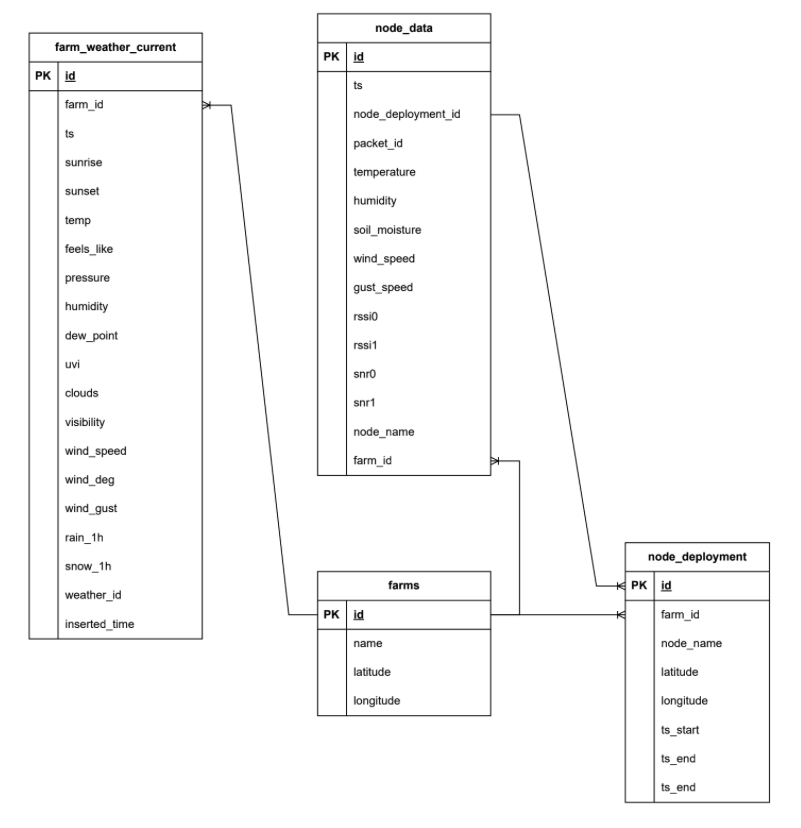
\includegraphics[width=0.8\textwidth]{contents/part-3/fig3/postgres_diagram.png}
    \caption{Table schema for postgreSQL database}
    \label{fig:db_schema}
\end{figure}

The database has four tables:

\begin{itemize}     
      \item farms: this holds a list of where the nodes are (or have been)
      deployed. The longitude and latitude of the farm is then used in API calls
      to OpenWeather (more on this below) which is used to fetch current and
      forecasted weather data.
      \item node\_deployment - This holds the precise longitude and latitude of
      each node as well as information on when the deployment started and ended.
      If the nodes are moved then this table is updated with new information.     
      \item node\_data - Holds the full set of readings from each node.    
      \item farm\_weather\_current - Holds current weather information from API
      calls to OpenWeather taken every 10 minutes and is strictly used to train
      the machine model explained in the machine learning section.
 \end{itemize} 


\subsection{Building an API}

With the database configured, I then developed a backend API using TypeScript
\cite{typescript}, Node.js \cite{nodejs}, and Express \cite{express}. This
service is responsible for interpreting incoming HTTP requests and performing
corresponding database operations - it is essentially the bridge between the
gateway hardware and the database. In addition to handling sensor data, the
service also integrates with an external weather API in order to retrieve both
current conditions and forecast data, which are then stored alongside the
locally collected sensor readings as explained in Section \ref{sec:database}.

The API inserts data into the database when it receives a POST request. The body
of the POST request contains a JSON body which is parsed, processed and added to
the database by the API. Data can be retrieved for display by the frontend using
a GET request.

The entire api is written using TypeScript. TypeScript is JavaScript with added
syntax that forces strong typing and features to enable error catching earlier
on. When TypeScript is compiled it produces a JavaScript file which contains the
actual code that is then executed. The main benefit of TypeScript is that it
leads to much more robust code with vastly fewer typing errors that vanilla
JavaScript can often let slip by. As I needed my API to have constant up time
and reliably insert and select from my database this made TypeScript ideal for
this application.

On top of TypeScript I used Node.js and the Express framework. Node.js allows
JavaScript to run on the server instead of inside a client browser, which lets
the project share a single language (i.e. JavaScript) across frontend and
backend development. It is well suited to creating APIs that handle many
simultaneous HTTP requests while calling on external APIs. This is because Node
runs asynchronously: when slow database queries are being executed Node will
continue listening and processing further requests. This non-blocking behaviour
means Node can handle large numbers of concurrent requests at the same time.
Additionally the node package manager (called with npm) has a large set of
useful libraries and allows my project to be rapidly set up on new computers
without having to retrieve required packages from different sources.

Express is a framework specific to Node.js that gives useful tools for creating
the API endpoints. I used express to write my request-handling functions for
each URL endpoint. These functions process incoming HTTP requests to the
endpoint and then execute the SQL query associated with that endpoint. Instead
of constantly opening new connections with the database I used the pg.Pool
library to pool requests together on the same connection. This helped to improve
the speed of SQL lookups and inserts helping requests to be executed faster,
which in turn improved the perceived performance of the webapp.

In total my api has five endpoints:

\begin{itemize}
  \item POST '/api/database/insert-node-data' - This endpoint is used by the
  gateway to fill the database with sensor data. When a valid HTTP request posts
  to this endpoint the JSON in the body of the request is parsed and inserted
  into the node\_data table. This endpoint has been included in
  \ref{app:api-endpoint} as an example.
  \item POST '/api/database/insert-weather-data' - This endpoint is used to
  insert general weather data from the OpenWeather API into the relevant table.
  The backend calls this every 10 minutes to collect the latest general weather
  data.
  \item GET '/api/database/select-latest' - This endpoint sends the latest
  sensor data from the node\_data table to the computer that sent the GET
  request. It is used by the front end to display current weather data.
  \item GET '/api/database/select-node-range' - This endpoint sends back the
  range of sensor data that is specified in the request body. It is used by the
  front end to build chart data.
  \item GET '/api/database/forecast' - This endpoint is used by the frontend to
  retrieve the latest forecast model data from the backend.
\end{itemize}

\subsection{Security}

Security was important in the design of the backend API as the end points are
exposed to the internet and thus any internet connected device is able to call
these. Therefore I had to take steps to prevent erroneous calls (such as from
bots) to my API endpoints which could insert data incorrectly or scrape the
contents.

\subsubsection{Environment variables}
The first step I took was to use environment variables inside Render to hide
sensitive information such as API keys and passwords. These variables are hidden
from any source documents and are injected separately at deploy time. This
prevents the information from leaking into the public domain.

\subsubsection{Bearer tokens}
Then I needed to prevent any unauthorised machine attempting to perform API
calls on my backend. The approach I took to this was to follow guidelines set
out in RFC 6750 related to the use of 'Bearer tokens' (essentially a password
check) \cite{rfc6750}. For this I checked that all incoming HTTP requests to my
API had an 'Authorization' line in their headers. I then checked whether the
string token after this matched the SECRET\_WORD variable in my environment
variables. Any request to the database without the correct header and token is
automatically rejected.

\subsubsection{Protecting against SQL injection}
Finally in case those security measures are not sufficient and a malicious actor
gets access to my API end points I then added protections against SQL
injections. SQL injections are a technique where an attacker can try to
manipulate a database by sending a crafted input that alters the intended
purpose of the endpoint.

For example if my API end point was designed to allow selections from a database
it might naïvely allow queries such as this:

\verb|SELECT ${httpBody.column} FROM ${httpBody.table_name};|

Expecting the \verb|httpBody| to contain a JSON with \texttt{column = "*"} and
\texttt{table\_name = "node\_data"}, for instance. 

However, if someone were to name their column as \texttt{"*"} and their
table\_name as \texttt{"node\_data; DROP TABLE node\_data;"} the effective
command would change to:

\verb|SELECT * FROM node_data; DROP TABLE node_data;|

This command would then select the data as intended before completely destroying
the table and all of its data. To prevent this from happening I whitelisted
valid inputs like so (psuedo-code for clarity);

\begin{verbatim}
const white_listed_columns = new Set('*');

const white_listed_tables = new Set('node_data');

if (!white_listed_tables.has(httpBody.table_name) 
    or !white_listed_columns.has(httpBody.column)) {
    return 404 error;
}
\end{verbatim}

\subsection{Weather API integration}

The weather API I settled on using to help build data for the forecasting
function of the webapp was the One Call API 3.0 by OpenWeather
\cite{openweatherAPI}. This API offers current weather data at a 10 minute
resolution as well as 48 hour ahead hourly and 8 day ahead daily weather
forecasts. The API permits up to 1000 calls per day before separate payment is
required. As I would only be requesting one current weather data reading and one
forecast data reading on 10 minute intervals I would only put through 288
requests per day which is well within the free limits.

To set up automatic API retrieval from my backend to the weather API I used the
node-cron library \cite{node-cron} to set up a 10 minute job on my host server.
This then called related functions to get both current and forecasted data for
use with my machine learning model.

\section{Frontend webapp}\label{sec:front-end}

\subsection{Design choices}

Before creating the frontend, I reviewed a handful of websites that display
weather and other data—including the Met Office, BBC Weather, and Apple
Weather—and informally discussed the preferred designs with peers.

\begin{figure}[H]
    \centering
    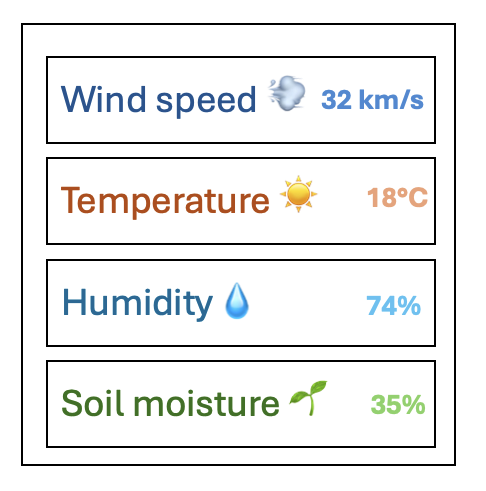
\includegraphics[width=0.3\textwidth]{contents/part-3/fig3/paper-prototype.png}
    \caption{Initial paper prototype for webapp with live information shown in clickable boxes}
    \label{fig:paper-prototype}
\end{figure}

Ultimately, I settled on a tile-based design similar to the paper prototype in
Figure \ref{fig:paper-prototype}, as this offered a simple and intuitive way to
view all current information at a glance. The concept was for users to click on
any tile to load a detailed chart for that specific data type. The following
sections describe the technologies selected to achieve this. 

\subsection{Choice of language in webapp}

The frontend of my project is written in HTML, CSS and JavaScript, which is an
archetypal web development stack.

\subsection{PicoCSS}

PicoCSS is the library I used for the default styling of my webapp. I liked its
minimal and low distraction look which I thought was ideal for presenting data.
It also had good mobile to desktop scaling which meant my webapp (at least the
non-chart parts) worked on mobile and desktop with little work needed.

\subsection{Apache Echarts}

Apache Echarts is a JavaScript library that I have used to build the charts for
my webapp. Data for charts is fetched from the backend and then loaded into a
'series' object. Apache Echarts then renders the data series onto a graph with a
variety of options that I have chosen to improve data clarity.

\subsection{ Walkthrough of Webapp features}\label{sec:walkthrough}

\begin{figure}[H]
    \centering
    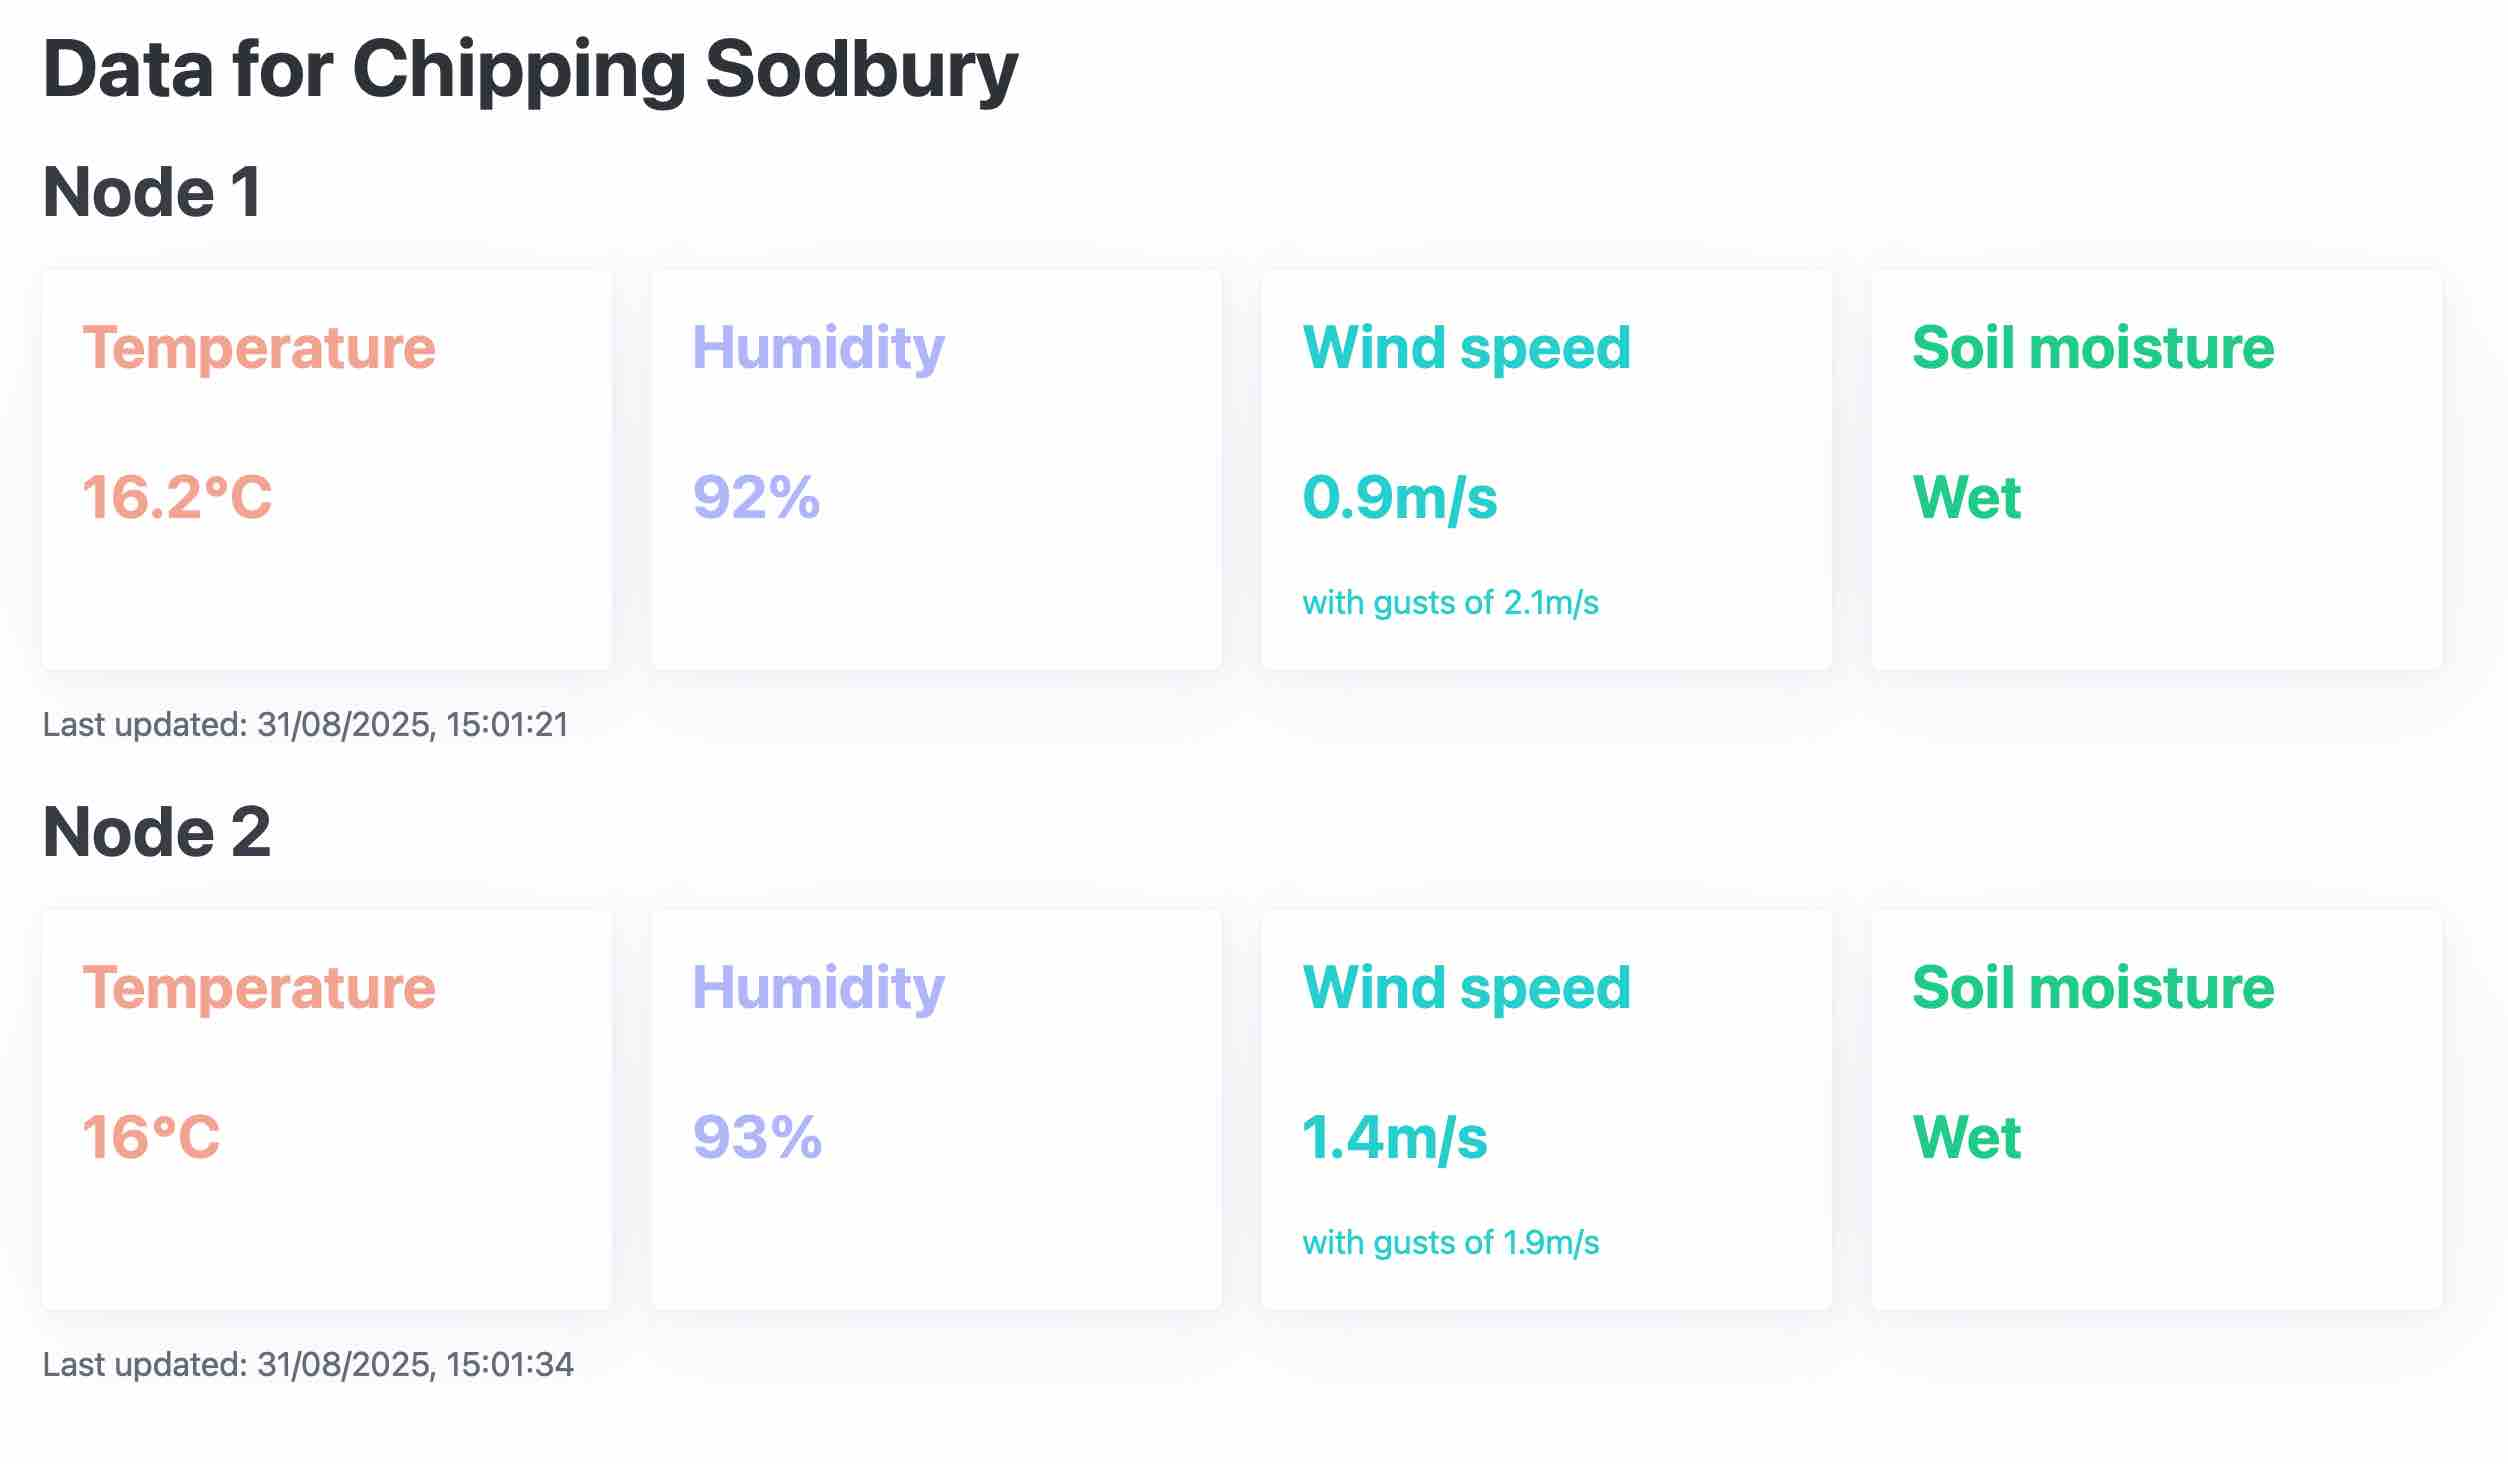
\includegraphics[width=0.8\textwidth]{contents/part-3/fig3/main-page.jpg}
    \caption{Main page of website showing current sensor readings}
    \label{fig:main-page}
\end{figure}

Figure \ref{fig:main-page} shows the main page of the webapp, which displays the
most recent readings for each node. A "Last updated" timestamp appears under
each set of readings, indicating how recently the data was received. Clicking on
any of these tiles opens a detailed chart for that specific metric.

\begin{figure}[H]
    \centering
    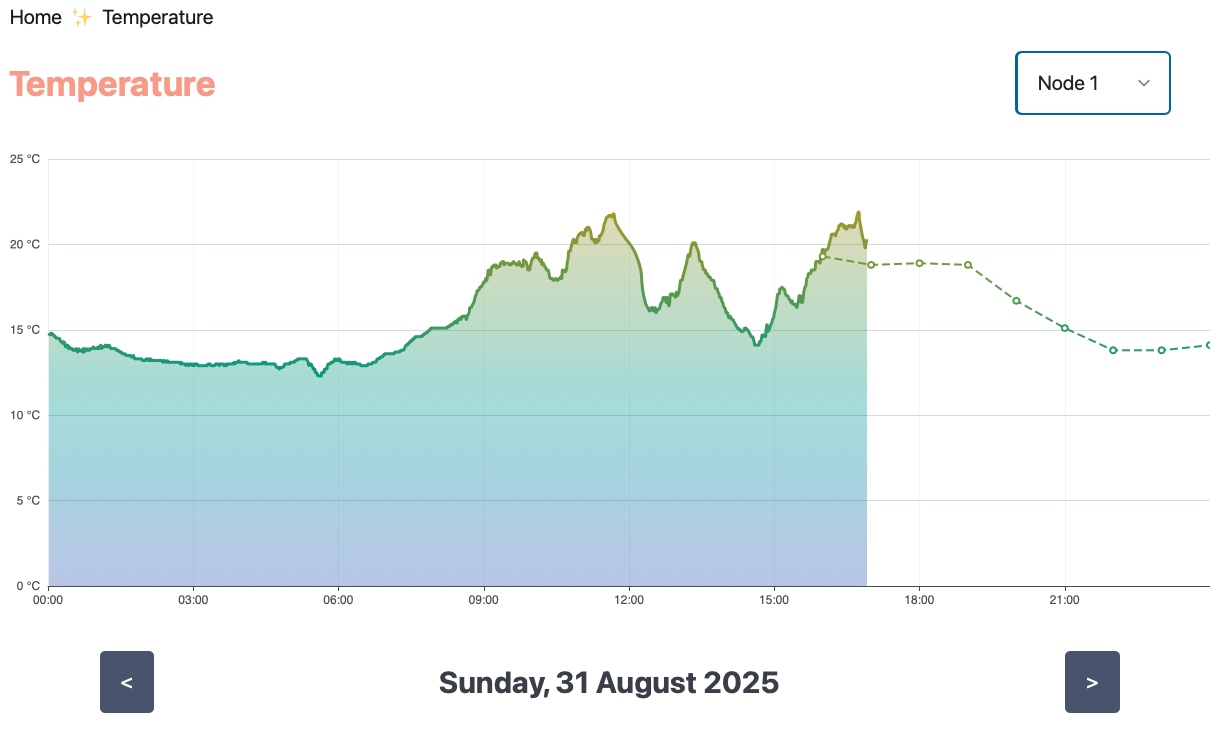
\includegraphics[width=0.8\textwidth]{contents/part-3/fig3/temperature-node-one.jpg}
    \caption{Temperature page with chart showing data for node 1}
    \label{fig:temp-page}
\end{figure}

The temperature page in Figure \ref{fig:temp-page} features a colour gradient
across the temperature range, with warmer values appearing more reddish and
cooler values more bluish. This is generated by the visualMap() function in
Echarts and provides the user with a quick visual cue of the current conditions.

\begin{figure}[H]
    \centering
    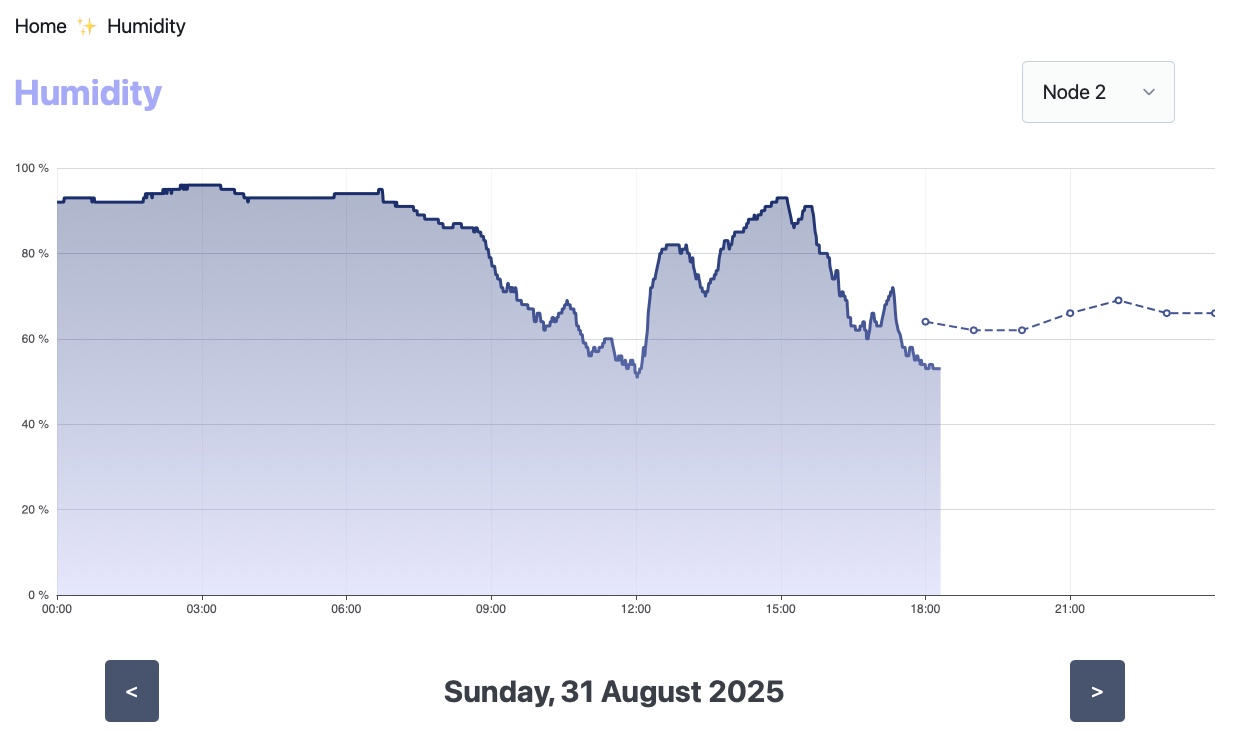
\includegraphics[width=0.8\textwidth]{contents/part-3/fig3/humidity-node-two.jpg}
    \caption{Humidity page with chart showing data for node 2}
    \label{fig:humidity-page}
\end{figure}

The Humidity page in Figure \ref{fig:humidity-page} similarly has a gradient
applied. Another noteworthy page element is the drop down menu in the top right,
which allows the user to switch the view between "Node 1", "Node 2", and
"Compare". Selecting an option updates the chart to show the corresponding
dataset, with "Compare" displaying a combined view of both nodes.

\begin{figure}[H]
    \centering
    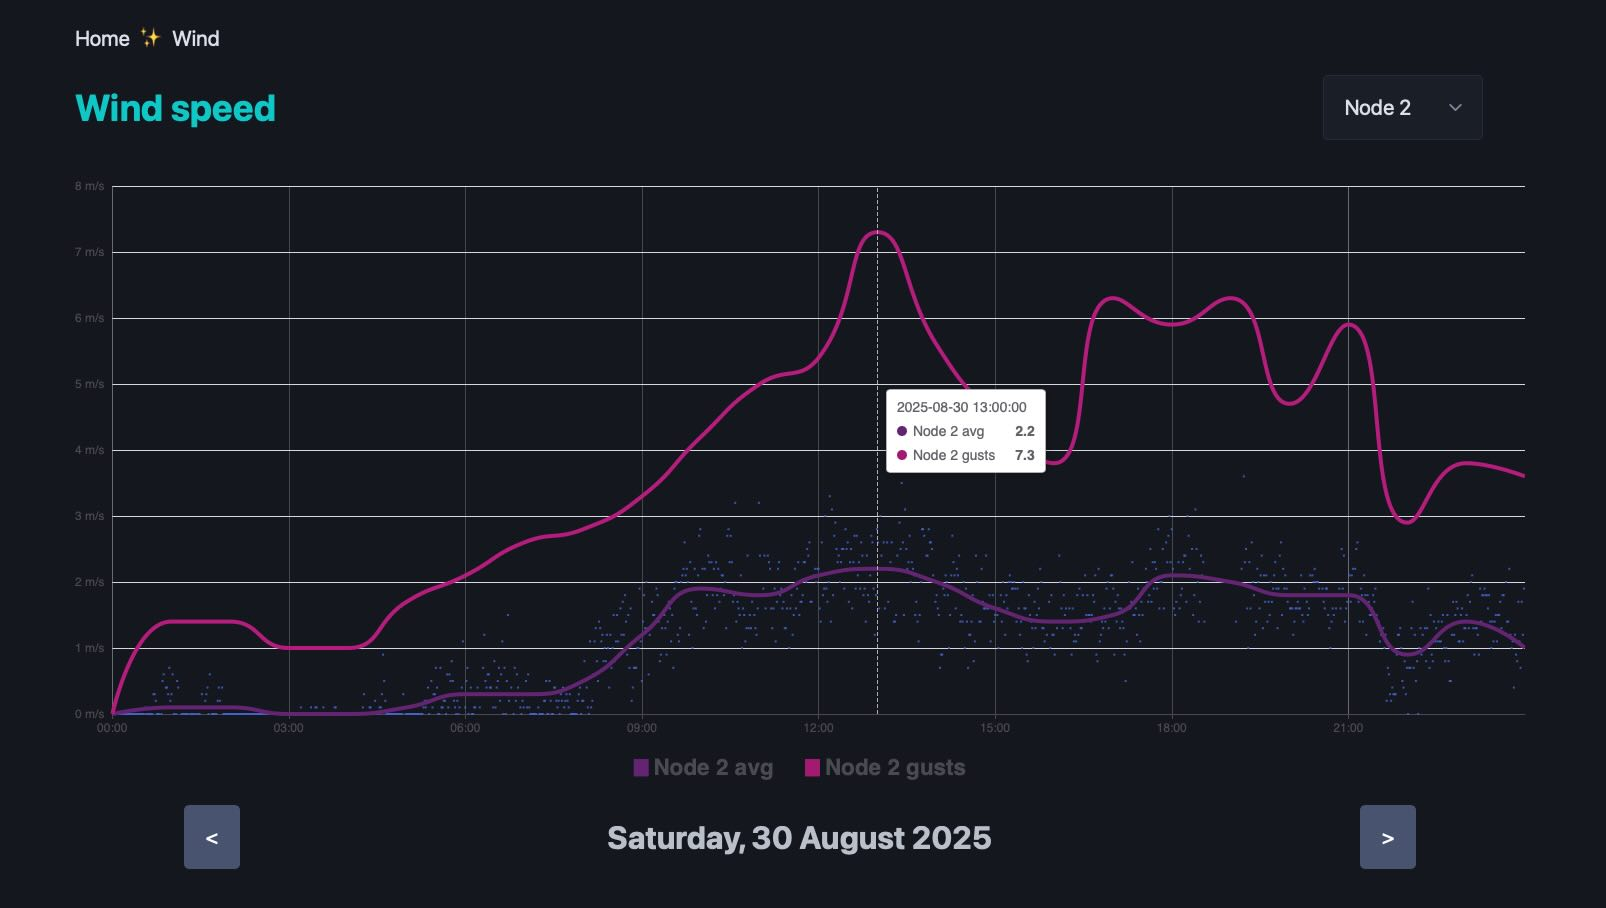
\includegraphics[width=0.8\textwidth]{contents/part-3/fig3/wind-speed-tooltip.jpg}
    \caption{Wind page with chart showing data for node 2}
    \label{fig:wind-page}
\end{figure}

Figure \ref{fig:wind-page} shows the webapp in dark mode. This is a feature of
the PicoCSS library, with the site's colour automatically adjusting to the
user's preferred appearance settings on their device.

Another key feature shown here is the tooltip. It appears when a desktop user
hovers over the chart or if a mobile user taps and drags. This displays the
precise numerical values on the chart at the point the user is hovering over.

Compared to the other chart types, the wind speed chart displays three data
series: a scatter plot of all raw wind readings (which is difficult to see in
the figure), a line for the hourly average wind speed, and another for the
highest gust speed recorded each hour. Also below the chart there is a legend
that allows the user to toggle the visibility of the average and gust speed
lines.

\begin{figure}[H]
    \centering
    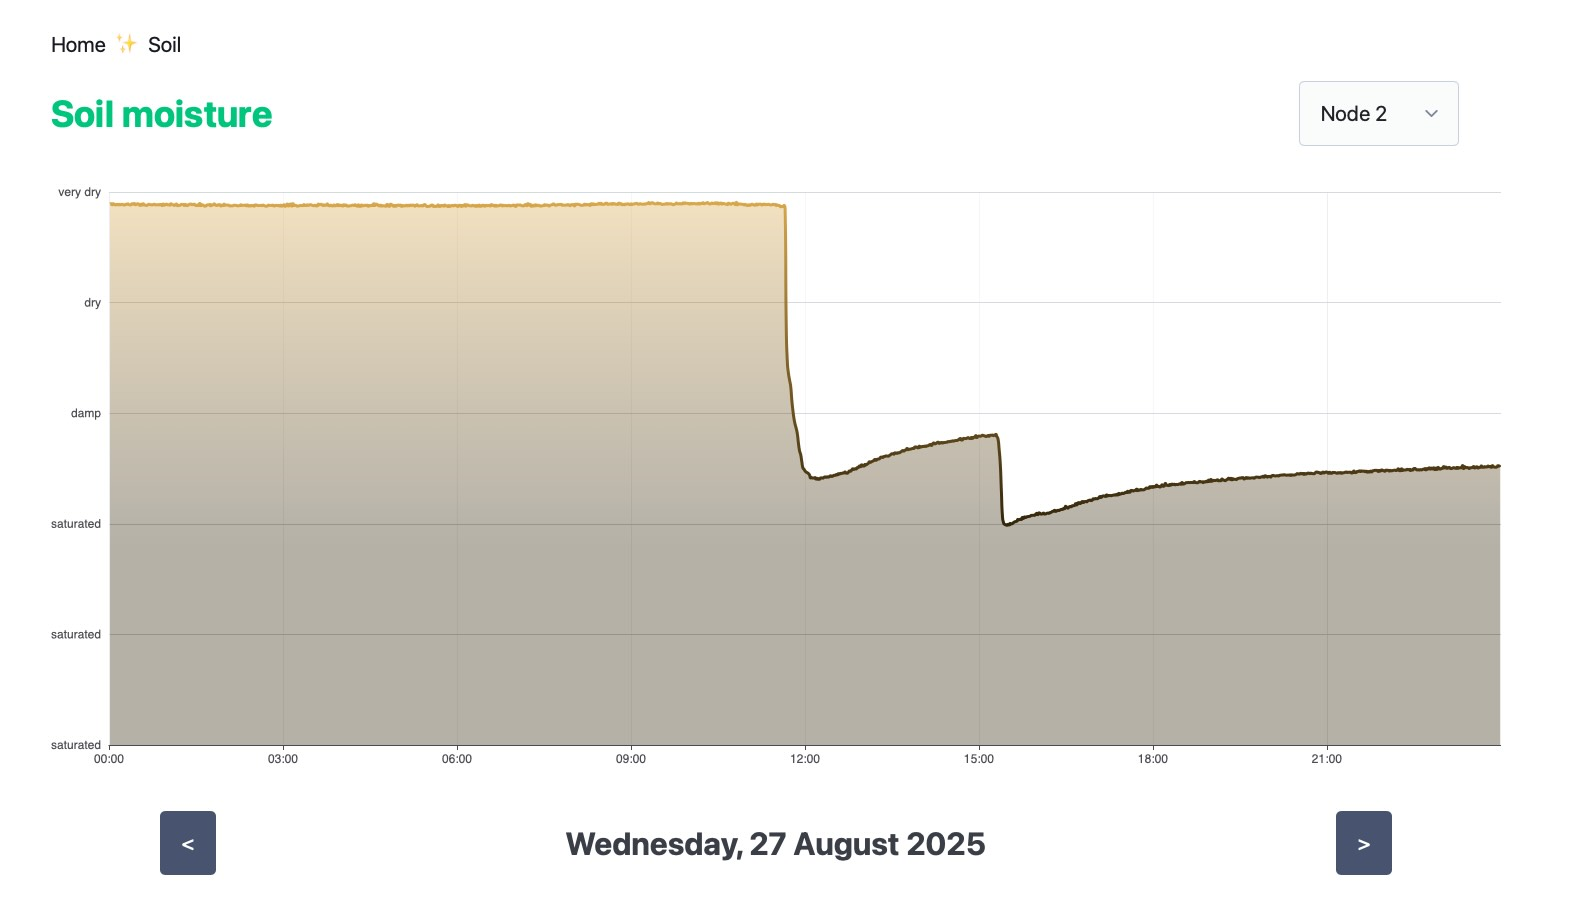
\includegraphics[width=0.8\textwidth]{contents/part-3/fig3/soil-moisture-light.jpg}
    \caption{Soil moisture page with chart showing data for node 1}
    \label{fig:soil-page}
\end{figure}

The soil moisture page in Figure \ref{fig:soil-page} shows the first day of
heavy rain fore the nodes. Other elements not already discussed include the
navigation bar in the top left that allows users to click back to home while
also showing the current page. There are also buttons to the left and right of
the date that allow the user to change date.

\begin{figure}[H]
    \centering
    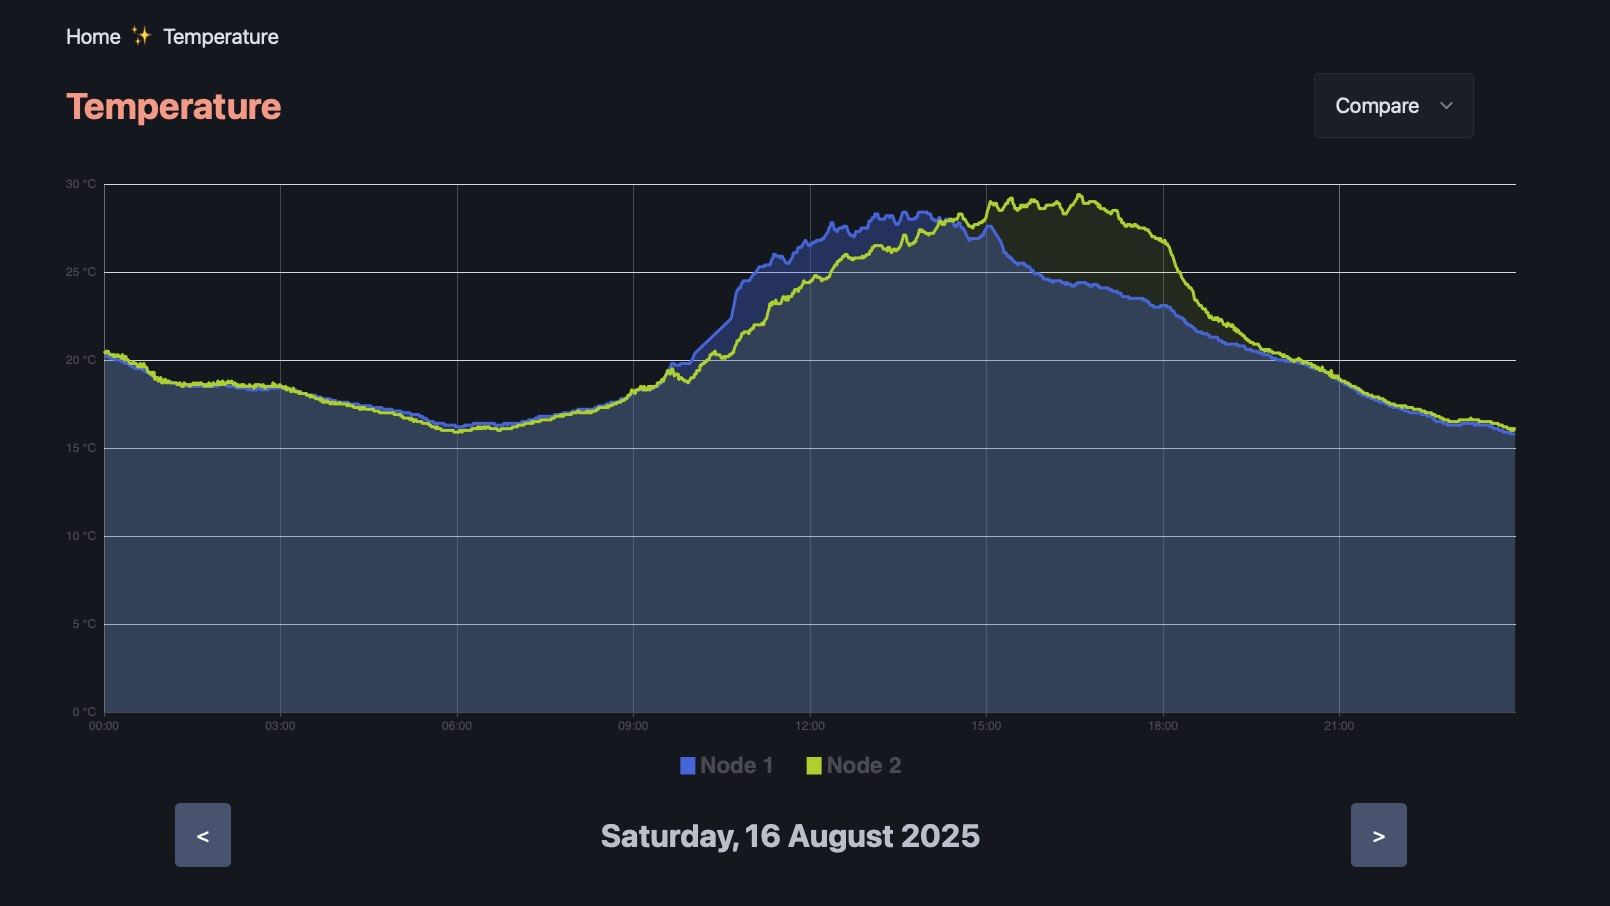
\includegraphics[width=0.8\textwidth]{contents/part-3/fig3/compare-mode.jpg}
    \caption{Temperature page showing comparison graph}
    \label{fig:compare-page}
\end{figure}

Figure \ref{fig:compare-page} shows the chart in comparison mode. In this view,
each node's data series is assigned a distinct colour to allow for easy visual
distinction between them.

\begin{figure}[H]
    \centering
    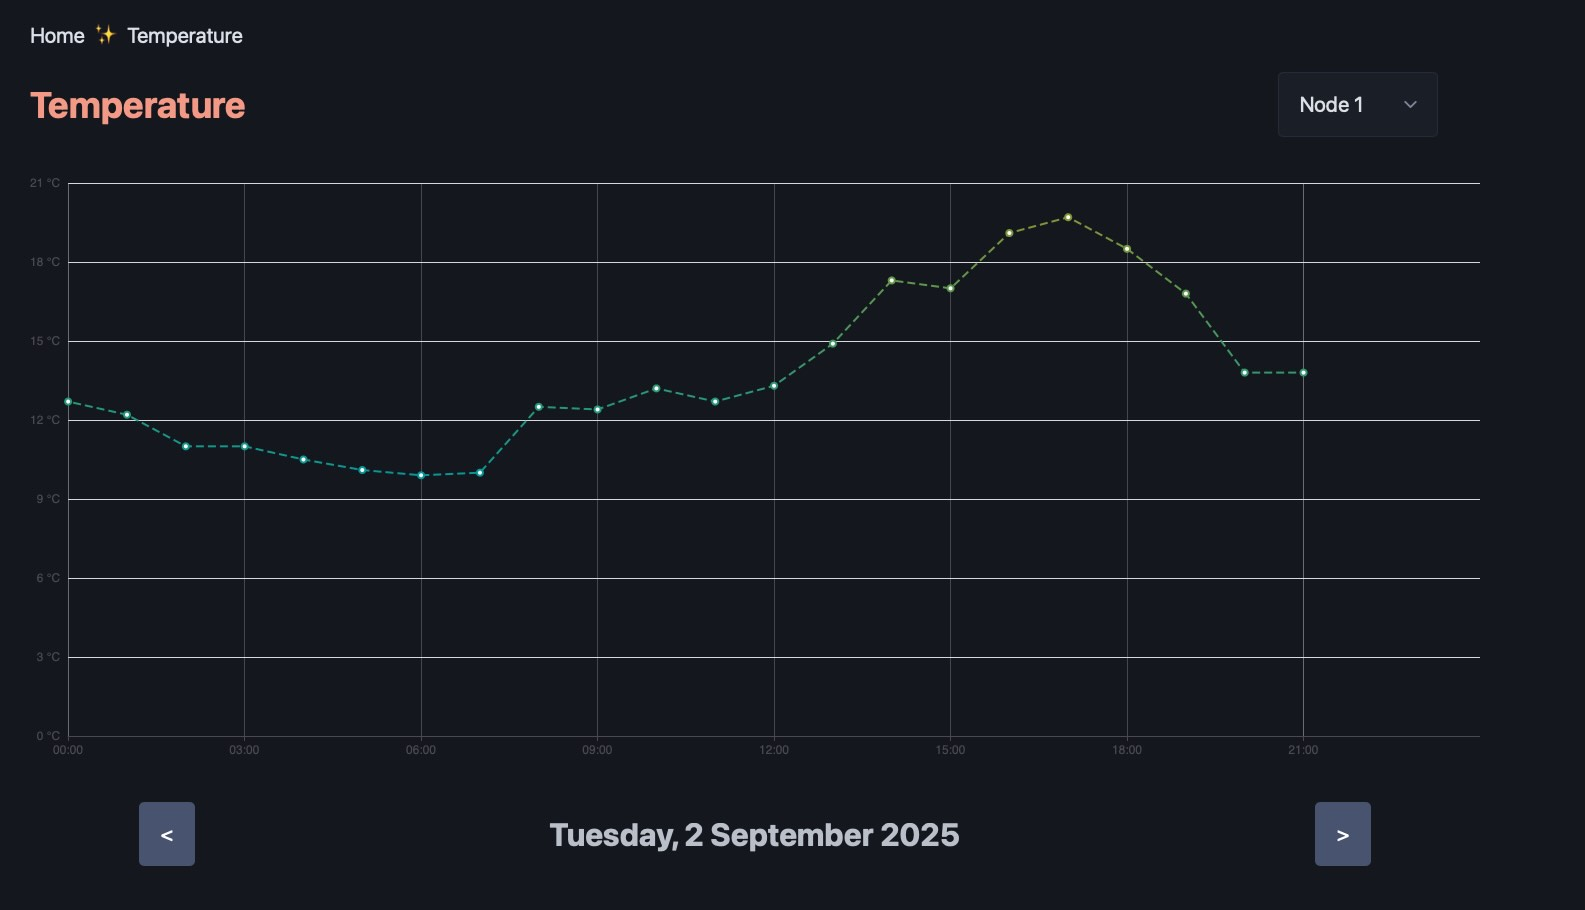
\includegraphics[width=0.8\textwidth]{contents/part-3/fig3/forecast.jpg}
    \caption{Temperature page for node 1 showing forecasted data}
    \label{fig:forecast-page}
\end{figure}

Finally Figure \ref{fig:forecast-page} shows the forecasting feature. This
applies to future time periods, presenting sensor data forecasted up to 48 hours
in advance by a machine learning model.

\subsection{Making the app mobile friendly}

I wanted the webapp to be accessible for both desktop and mobile users. What
tends to make this difficult is the fact that scaling on desktop and mobile is
normally very different. Mobile devices have a longer vertical axis while on
desktop it tends to be the reverse - so I needed to ensure elements were
reactive to the screen size of the viewer.

PicoCSS comes with much of this reactive formatting as standard on default HTML
elements (selection boxes, divs, titles, navigation bars etc). However
integrating Echarts was difficult as PicoCSS styles cannot directly apply to
this. I therefore took actions to improve the usability for mobile users, as
summarised below:

\begin{enumerate}
    \item Dynamic tooltip: The webapp can tell if the viewer is a touch screen
          and if so it will make the tool tip hover slightly away from the point
          of touch. While on desktop the user will want to hover over a
          datapoint and see the tool tip appear where they are hovering, on
          mobile the digit used to select may cover important tooltip
          information. By making sure the tooltip hovers slightly away from the
          selection this is no longer a problem.
    \item Dynamic chart and font size: Echarts comes with no standard method of
          resizing chart data depending on the size of the device viewing the
          chart. So I ensured that the size of the chart (including its font)
          would be drawn smaller on mobile devices and recalculated if the
          viewing size changes (i.e. if a desktop user shrinks the window size)
    \item Dynamic X axis: The interval between X axis ticks on mobile is 6 hours
        vs 3 hours on desktop, so that on mobile the view is less crowded.
    \item Dropdown menu for chart selection: I initially used a radio design for
        the chart type selection (like a multiple choice question) but quickly
        realised this was not a mobile friendly design choice as the scaled down
        buttons were very hard to click. I instead opted to use a drop down box
        as this was much easier to select on a mobile setting while still a well
        known element that users should be familiar with.
\end{enumerate}

One of the hardest pages to format well for mobile users was the wind sensor
comparison page as this is has many different series elements to display (two
wind averages and two gust averages). However from Figure \ref{fig:mobile-page}
we can see that all elements fit comfortably in frame despite the large number
of series and legend data.

\begin{figure}[H]
    \centering
    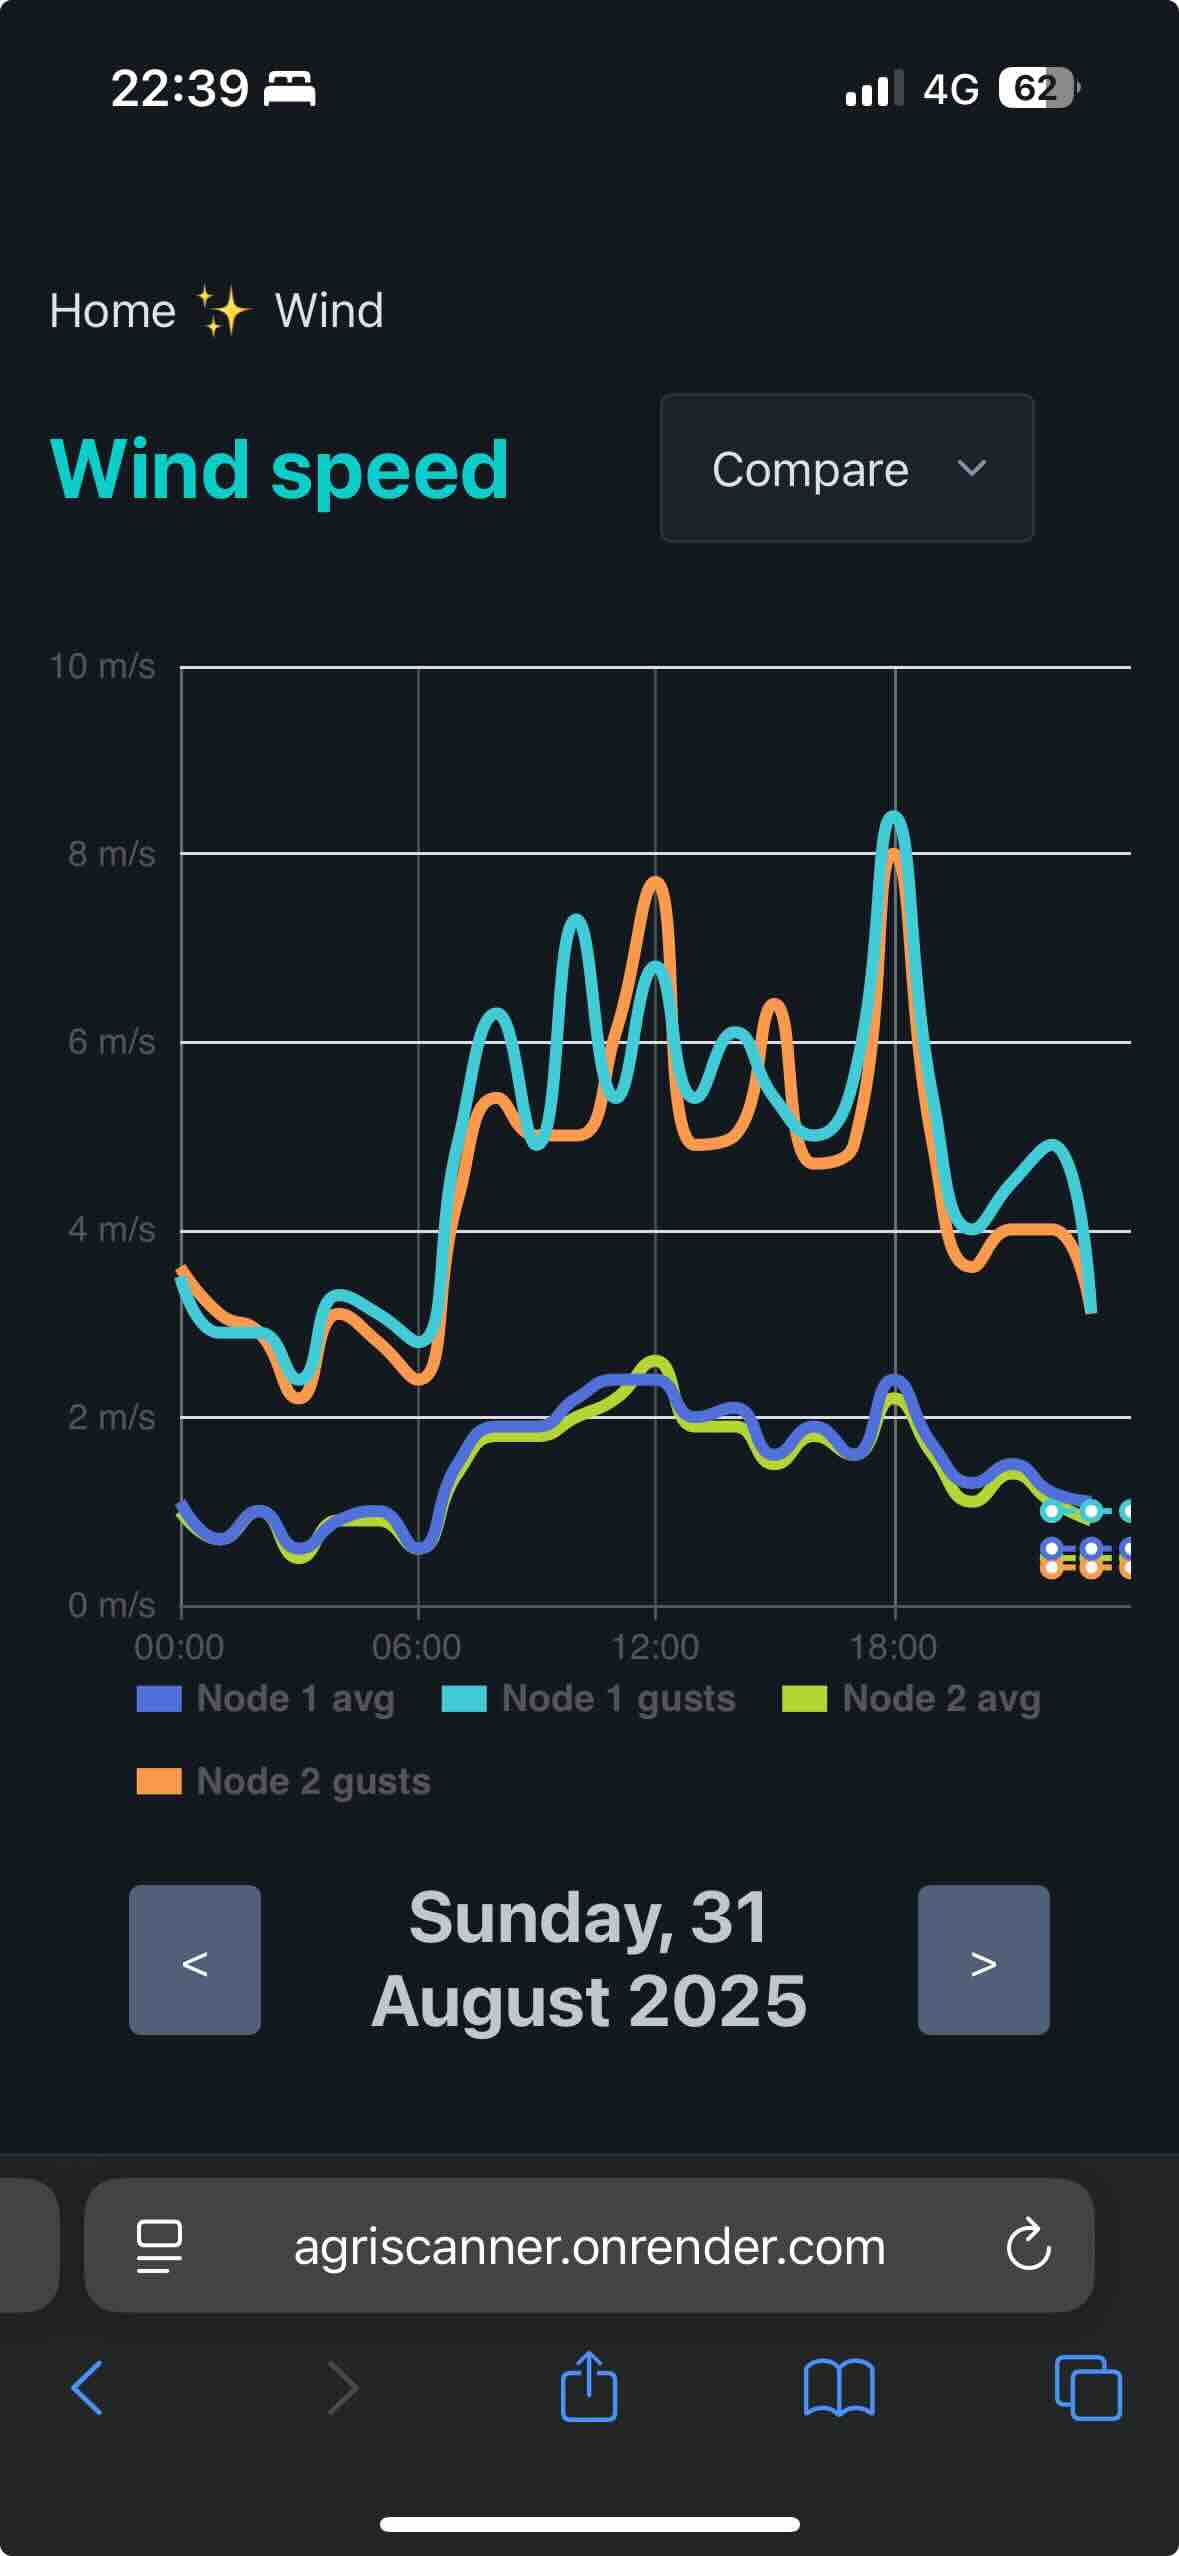
\includegraphics[width=0.3\textwidth]{contents/part-3/fig3/mobile-wind-speed-compare.jpeg}
    \caption{Mobile phone showing wind speed comparison chart}
    \label{fig:mobile-page}
\end{figure}


